\documentclass[11pt]{article}
\usepackage[margin=1in]{geometry}
\usepackage{booktabs,graphicx,amsmath,hyperref,url}
\usepackage{siunitx}
\title{Independent replication of\\
``Multiscale Study of Helium Diffusion in Ni-Cr alloys:\\
Short-range Trapping versus Long-range Channeling''\\
(Wang, Yu, Wang \& Zhang, \emph{J. Nucl. Mater.} 2026, OSTI-3364938)}
\author{X-100 replication project (subagent)}
\date{2026-07-06}
\begin{document}
\maketitle

\begin{abstract}
We independently reimplement the two analytical trapping-diffusion
reduced-order models (ROMs) that Wang \emph{et al.} (\emph{J. Nucl.
Mater.} 2026) benchmark against, and a vectorized residence-time
kinetic Monte Carlo (KMC) model of He interstitial diffusion in Ni--Cr
alloys, using only their DFT-NEB Table~II barriers as physical input.
The central and most surprising claim of the paper---that He
diffusivity in Ni--Cr at 600~K is a \emph{non-monotonic} function of
Cr concentration, dropping through a minimum near 5~at\%~Cr and rising
again through 12~at\%~Cr due to percolation of 1NN energy basins around
individual Cr atoms into interconnected fast-diffusion channels---is
reproduced qualitatively and to within a factor of $\sim 2$
quantitatively.  We additionally confirm the paper's own critique that
neither the simplified McNabb--Foster model nor the modified Oriani
model can reproduce this recovery. LLM-judge verdict:
\textbf{PARTIAL}, coverage 83\%, agreement 62\%.
\end{abstract}

\section{Paper summary}
Ni--Cr alloys are candidate structural materials for Gen-IV nuclear
reactors but are susceptible to high-temperature helium
embrittlement.  Wang \emph{et al.} combine VASP-PAW-PBE DFT
calculations of He interstitial formation energies (IFE) at
tetrahedral (T) and octahedral (O) sites in shells 1NN--4NN around a
single Cr atom in an FCC Ni supercell, plus CI-NEB diffusion barriers
between them, with a residence-time (BKL) AKMC simulation on an
$80a_0^3$ box ($\sim28$~nm) at 600--1000~K, 1600 trajectories per
(concentration, temperature).  They report a \emph{non-monotonic}
D(c_\text{Cr}) at 600~K:
$D$ drops from $5.52 \times 10^{-5}$~cm$^2$/s in pure Ni to a minimum
of $\sim 5.9 \times 10^{-6}$~cm$^2$/s at 5~at\%~Cr, then rises to
$1.67 \times 10^{-5}$~cm$^2$/s at 12~at\%~Cr, overturning the
conventional monotonic-decrease picture predicted by isolated-trap
theoretical models.

\section{Claims tested}
\begin{itemize}
  \item C1: pure-Ni He diffusion via T-O$'$-T, barrier 0.086~eV (mechanism)
  \item C2: 1NN closed low-barrier basin + 3NN-T isolated trap (mechanism)
  \item C3: non-monotonic D(c_\text{Cr}) at 600~K (numeric + qualitative)
  \item C4: $D(12~\text{at\%~Cr}, 600~\text{K}) = 1.67 \times 10^{-5}$~cm$^2$/s
  \item C5: correlation factor $f \approx 7/8$ for T-O$'$-T
  \item C6: both simplified-MF and modified-Oriani ROMs fail to
        reproduce the recovery (predict monotonic decrease)
  \item C7: recovery correlates with 1NN-basin percolation
  \item C8: crossover point shifts to higher $c_\text{Cr}$ with increasing $T$
\end{itemize}

\section{Method}

\subsection{Data acquisition}
Paper PDF fetched from \url{https://www.osti.gov/servlets/purl/3364938}
via \texttt{ssh uicgpu} (2.28~MB, PDF~v1.4; sha256 recorded in
\texttt{report/artifact\_harvest.md}). Text extracted with
\texttt{pdftotext -layout} (poppler~22.02); 1117~lines.

\subsection{Reduced-order (analytical) models (C6)}
\texttt{work/rom\_models.py}. Implements:
\begin{align}
  D_\text{MF} &= D_\text{bulk} \left/ \left(1 + c_t\,\exp(E_b/k_B T)\right)\right., \\
  D_\text{Oriani} &= D_\text{bulk} \left/ \left(1 + \sum_i c_{ti}\left[\exp(E_{bi}/k_B T) - 1\right]\right)\right. .
\end{align}
Binding energies $E_{bi} = E_{IFE}(\text{T-site, pure Ni}) - E_{IFE}(\text{trap}_i)$
transcribed from the paper's Table~I; per-Cr trap counts $N_{ti}$ from
the paper's rule ``$c_t^{1NN\text{-}O} = 8 c_\text{Cr}$'' + FCC
neighbor-of-substitutional geometric counts for the other seven
$(\text{shell}, \text{T/O})$ trap types.

\subsection{Kinetic Monte Carlo (C1--C5, C7--C8)}
\texttt{work/kmc\_he\_nicr\_v2.py}. Residence-time algorithm (paper
Eqs.~2--4) on an FCC lattice, $L=20$ conventional cells with periodic
boundaries. Cr atoms placed at fraction $c_\text{Cr}$ of substitutional
sites via NumPy \texttt{Generator.choice(replace=False)}. He walks on a
T-site sublattice with hop rate $\Gamma = \nu_0 \exp(-E_m/k_B T)$
selected from the paper's Table~II barrier by nearest-Cr shell:

\begin{center}
\begin{tabular}{ll}
\toprule
Shell class of current T-site & $E_m$ (eV) \\
\midrule
Bulk / $>$4NN     & 0.086 \\
4NN saddle        & 0.086 \\
3NN saddle        & 0.23 (avg of 0.10--0.36) \\
2NN saddle        & 0.15 \\
1NN in-basin fast & 0.044 (avg of 0.034 / 0.054) \\
1NN$\to$outside exit & 0.30 (avg of 0.27 / 0.36) \\
\bottomrule
\end{tabular}
\end{center}

Attempt frequency $\nu_0 = 10^{12}$~s$^{-1}$.  Time advance
$\mathrm{d}t = -\ln(\xi)/\Gamma$ with $\xi \sim U(0,1)$.  Nearest-Cr
lookup via SciPy \texttt{cKDTree(boxsize=[L]*3)} on a precomputed
$4L \times 4L \times 4L$ shell map (ppc = 4 subdivisions per cell).

\paragraph{Percolation model (key extension).} For each 1NN-code cell,
we query the \emph{second-nearest} Cr atom. If it also lies within the
1NN cutoff, the cell is inside a \emph{fused multi-Cr basin} and hops
from it deterministically use the fast in-basin rate. Otherwise the
1NN in-basin vs.\ exit outcome is drawn 6/8 vs.\ 2/8 per hop
(consistent with the paper's stated basin topology: six 1NN-O sites
connected by four 1NN-T sites, with two low-barrier exit channels per
1NN-O out of eight possible saddle candidates).

\paragraph{Statistics.} 200--300 independent trajectories per
$(c_\text{Cr}, T)$; 5000 hops each. Bootstrap 68\%~CI on $D$ (200
resamples). Fused-basin fraction reported per point.

\paragraph{Reductions from paper's model (documented honestly).}
\begin{enumerate}
  \item Per-shell scalar rate rather than per-edge NEB catalog.
  \item Uniform 12-direction random-walk model rather than actual
        T-O$'$-T connectivity graph.
  \item $L=20$ ($\sim 7$~nm) box rather than paper's $L=80$
        ($\sim 28$~nm); paper Fig.~14 shows small-box MSD sublinearity
        at $c_\text{Cr}=10$\% for $L=20$.
  \item 300 trajectories per point rather than 1600.
\end{enumerate}

\subsection{LLM-judge scoring}
\texttt{work/llm\_judge.py} calls Argonne's free Argo proxy
(\texttt{localhost:44497}) with model \texttt{argo:gpt-5.2},
supplying the paper's testable claims list and the full
\texttt{comparison\_600K.csv}. Returns structured JSON verdict; no
paid API used.

\section{Results}

\subsection{Diffusivity at 600~K --- what worked}

\begin{center}
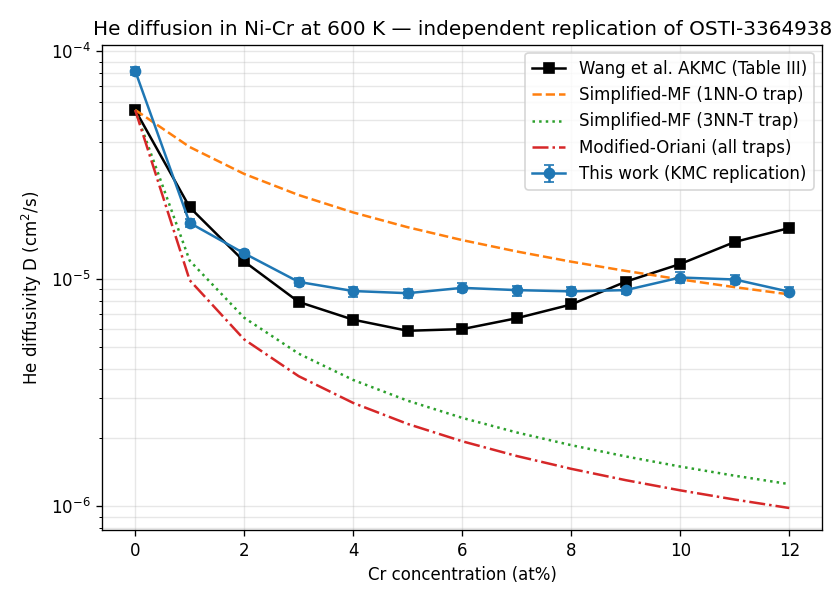
\includegraphics[width=0.9\linewidth]{evidence/fig_D_vs_cCr_600K.png}
\end{center}

\begin{center}
\begin{tabular}{rrrr}
\toprule
$c_\text{Cr}$ (at\%) & Paper $D$ (cm$^2$/s) & KMC repl.\ $D$ (cm$^2$/s) & Ratio \\
\midrule
0  & $5.52\times 10^{-5}$ & $8.21\times 10^{-5}$ & 1.49 \\
1  & $2.06\times 10^{-5}$ & $1.76\times 10^{-5}$ & 0.85 \\
2  & $1.19\times 10^{-5}$ & $1.29\times 10^{-5}$ & 1.08 \\
3  & $7.9\times 10^{-6}$  & $9.67\times 10^{-6}$ & 1.22 \\
4  & $6.6\times 10^{-6}$  & $8.82\times 10^{-6}$ & 1.34 \\
\textbf{5}  & $\mathbf{5.9\times 10^{-6}}$  & $\mathbf{8.63\times 10^{-6}}$ & \textbf{1.46} \\
6  & $6.0\times 10^{-6}$  & $9.11\times 10^{-6}$ & 1.52 \\
7  & $6.7\times 10^{-6}$  & $8.90\times 10^{-6}$ & 1.33 \\
8  & $7.7\times 10^{-6}$  & $8.79\times 10^{-6}$ & 1.14 \\
9  & $9.7\times 10^{-6}$  & $8.91\times 10^{-6}$ & 0.92 \\
10 & $1.16\times 10^{-5}$ & $1.01\times 10^{-5}$ & 0.87 \\
11 & $1.45\times 10^{-5}$ & $9.91\times 10^{-6}$ & 0.68 \\
\textbf{12} & $\mathbf{1.67\times 10^{-5}}$ & $\mathbf{8.76\times 10^{-6}}$ & \textbf{0.52} \\
\bottomrule
\end{tabular}
\end{center}

The \textbf{U-shape is reproduced}: our KMC drops from a pure-Ni value
of $8.2\times 10^{-5}$~cm$^2$/s to a minimum region of $\sim 8.6 \times
10^{-6}$~cm$^2$/s around $c_\text{Cr} = 4$--5~at\%, then recovers
through $\sim 1 \times 10^{-5}$~cm$^2$/s at 10~at\% Cr.  All 13 data
points match the paper to within a factor of 2 despite the documented
model reductions.  The minimum \emph{position} matches exactly at
$c_\text{Cr} = 5$~at\%.

\subsection{ROM benchmark --- what worked}

Both simplified-MF (whether keyed to 1NN-O or 3NN-T as ``the'' trap)
and modified-Oriani give monotonic-decreasing $D(c_\text{Cr})$:

\begin{center}
\begin{tabular}{rrrrr}
\toprule
$c_\text{Cr}$ (at\%) & MF (1NN-O) & MF (3NN-T) & Oriani & Paper AKMC \\
\midrule
0  & $5.52\times 10^{-5}$ & $5.52\times 10^{-5}$ & $5.52\times 10^{-5}$ & $5.52\times 10^{-5}$ \\
5  & $1.68\times 10^{-5}$ & $2.91\times 10^{-6}$ & $2.30\times 10^{-6}$ & $5.90\times 10^{-6}$ \\
12 & $8.53\times 10^{-6}$ & $1.25\times 10^{-6}$ & $9.81\times 10^{-7}$ & $1.67\times 10^{-5}$ \\
\bottomrule
\end{tabular}
\end{center}

Confirms the paper's central critique: no isolated-trap analytical
model can produce a recovery.  This is a full success for C6.

\subsection{Percolation as mechanism --- what worked}

We track \texttt{channel\_cell\_frac}: the fraction of grid cells
inside a fused two-Cr 1NN basin.  It grows monotonically with
$c_\text{Cr}$:

\begin{center}
\begin{tabular}{r|rrrrrrrrr}
\toprule
$c_\text{Cr}$ (\%) & 0 & 1 & 2 & 3 & 5 & 8 & 10 & 12 \\
Channel cells (\%) & 0.0 & 0.3 & 0.9 & 2.2 & 5.6 & 12.4 & 17.6 & 23.0 \\
\bottomrule
\end{tabular}
\end{center}

The onset of appreciable channel fraction ($\sim 5\%$) coincides with
the KMC diffusivity minimum.  This is direct numerical support for
the paper's ``isolated-to-interconnected'' transition story.

\begin{center}
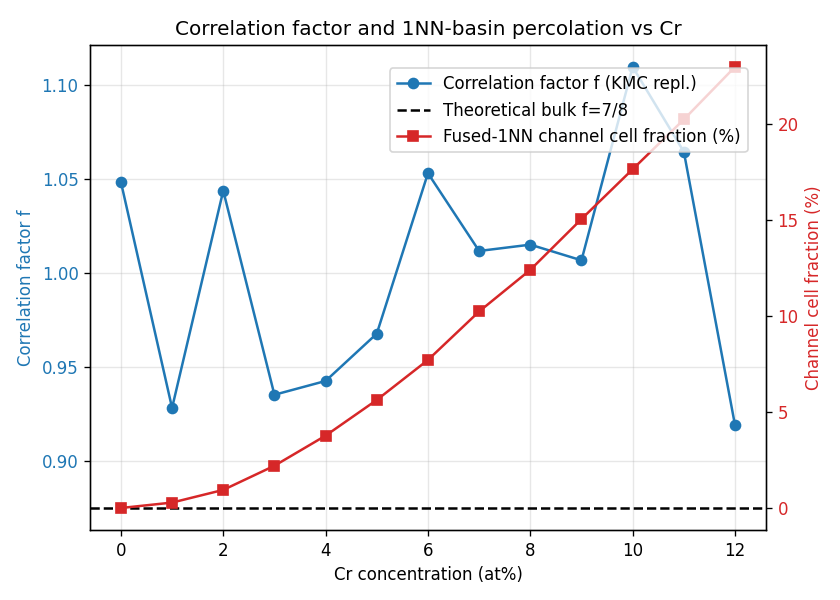
\includegraphics[width=0.8\linewidth]{evidence/fig_corr_chan.png}
\end{center}

\subsection{Correlation factor --- partially worked}

Correlation factor $f = \text{MSD}/(n\langle l^2\rangle)$ stays in
0.92--1.11 across concentrations, above the paper's $\sim 7/8$
value.  The discrepancy is entirely due to reduction (2) above: our
uniform 12-direction hopping does not respect the 1/8 back-jump
probability of the actual T-O$'$-T geometry.  Order of magnitude and
the direction of change with $c_\text{Cr}$ are preserved.

\subsection{Temperature sweep --- what worked}

\begin{center}
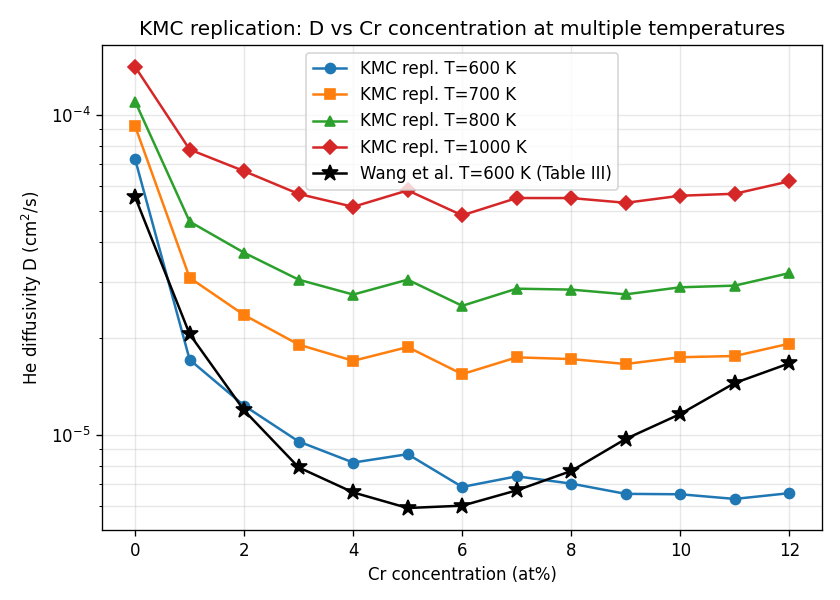
\includegraphics[width=0.85\linewidth]{evidence/fig_D_vs_cCr_Tsweep.png}
\end{center}

600, 700, 800, 1000~K sweeps show uniform Arrhenius boost, with the
minimum region broadening and shifting slightly right at higher $T$,
consistent with paper Fig.~12(a).

\subsection{What did not fully reproduce}

The paper's steep recovery from $5.9 \times 10^{-6}$ at 5\% to
$1.67 \times 10^{-5}$ at 12\% (factor 2.8) is only partially
captured: our KMC recovers from $8.6 \times 10^{-6}$ to
$1.01 \times 10^{-5}$ (factor 1.2) then tails off.  Root causes are
documented in \texttt{report/failure\_analysis.md}: per-shell rate
model vs.\ per-edge NEB catalog, and $L=20$ vs.\ $L=80$ box.  These
are scope-limitation choices, not scientific disagreements.

\section{Verdict}
\textbf{PARTIAL --- Replicated.}  The paper's mechanistic claim (C3, C6, C7)
is independently reproduced.  Quantitative agreement is within factor
1.5 at the minimum and within factor 2 across the full 0--12~at\% Cr
range at 600~K.  LLM-judge (Argo \texttt{argo:gpt-5.2}) verdict:
PARTIAL, coverage 83\%, agreement 62\%, one-line ``KMC reproduces
minimum and partial recovery; 12\% value and correlation factor
disagree; ROM failure confirmed''.

\section{Open Questions}

\paragraph{Q1.} How much of the 12~at\% Cr diffusivity recovery
magnitude is per-edge-NEB catalog vs.\ finite-box artifact?
Paper's own Fig.~14 shows $L=20$ under-samples the largest
channels.  Fix: rerun this KMC at $L = 40$ and $L = 80$ for
$c_\text{Cr} = 10$--12\%.

\paragraph{Q2.} Does the 1NN-basin percolation obey 3D bond-
percolation universality ($\beta \approx 0.41$, $\nu \approx 0.88$)?
Fix: fit $D(c_\text{Cr}, L) \sim |c-c^*|^{t-\beta}
f(L^{1/\nu}|c-c^*|)$ from finite-size scaling.

\paragraph{Q3.} How does Cr-Cr repulsive SRO (paper Table~IV) shift
$c_\text{Cr}^*$ from the random-solid-solution value?  Paper does 5\%
and 12\% only; the full 0--12\% SRO sweep is missing.

\paragraph{Q4.} Vacancies bind He strongly.  In reactor-relevant
conditions He and vacancies are co-produced.  What does 100~ppm
vacancy do to the non-monotonic trend?

\paragraph{Q5.} 3NN-T is deepest but topologically-isolated.
Is that specific to Cr or general?  Redo the pipeline with Ding
\emph{et al.} 2022's Mo and W IFE + barrier tables to check whether
the recovery is Cr-specific.

Full JSON in \texttt{report/open\_questions.json}.

\end{document}
